\documentclass[11pt]{article}
\usepackage[margin=1in]{geometry}
\usepackage[T1]{fontenc}
\usepackage[utf8]{inputenc}
\usepackage{lmodern}
\usepackage{microtype}
\usepackage{amsmath,amsfonts}
\usepackage{booktabs}
\usepackage{graphicx}
\usepackage[numbers,sort&compress]{natbib}
\usepackage[colorlinks=true,linkcolor=black,citecolor=black,urlcolor=black]{hyperref}
\usepackage{url}
\graphicspath{{../results/figures/}{../results/demo/}}

\title{Mikiri: Learned Stopping and Exact Search Memory\\ on a Frozen Go Engine}
\author{Taka Khoo\\[2pt]
Thayer School of Engineering, Dartmouth College\\
\texttt{taka.khoo.th@dartmouth.edu}}
\date{October 2026}

% Generated by experiments/paper_tables.py. Do not edit.
\newcommand{\mainGames}{\textbf{??}}
\newcommand{\mainRecord}{\textbf{??}}
\newcommand{\mainScore}{\textbf{??}}
\newcommand{\mainElo}{\textbf{??}}
\newcommand{\mainEloLo}{\textbf{??}}
\newcommand{\mainEloHi}{\textbf{??}}
\newcommand{\mainVisits}{\textbf{??}}
\newcommand{\mainRestart}{\textbf{??}}
\newcommand{\mainEvals}{\textbf{??}}
\newcommand{\mainBaseEvals}{\textbf{??}}
\newcommand{\mainHitRate}{\textbf{??}}
\newcommand{\mainHitLate}{\textbf{??}}
\newcommand{\mainMemory}{\textbf{??}}
\newcommand{\strictGames}{\textbf{??}}
\newcommand{\strictRecord}{\textbf{??}}
\newcommand{\strictScore}{\textbf{??}}
\newcommand{\strictElo}{\textbf{??}}
\newcommand{\strictEloLo}{\textbf{??}}
\newcommand{\strictEloHi}{\textbf{??}}
\newcommand{\strictVisits}{\textbf{??}}
\newcommand{\strictRestart}{\textbf{??}}
\newcommand{\strictEvals}{\textbf{??}}
\newcommand{\strictBaseEvals}{\textbf{??}}
\newcommand{\strictHitRate}{\textbf{??}}
\newcommand{\strictHitLate}{\textbf{??}}
\newcommand{\strictMemory}{\textbf{??}}
\newcommand{\pairedGames}{\textbf{??}}
\newcommand{\pairedRecord}{\textbf{??}}
\newcommand{\pairedScore}{\textbf{??}}
\newcommand{\pairedElo}{\textbf{??}}
\newcommand{\pairedEloLo}{\textbf{??}}
\newcommand{\pairedEloHi}{\textbf{??}}
\newcommand{\pairedVisits}{\textbf{??}}
\newcommand{\pairedRestart}{\textbf{??}}
\newcommand{\pairedEvals}{\textbf{??}}
\newcommand{\pairedBaseEvals}{\textbf{??}}
\newcommand{\pairedHitRate}{\textbf{??}}
\newcommand{\pairedHitLate}{\textbf{??}}
\newcommand{\pairedMemory}{\textbf{??}}
\newcommand{\memonlyGames}{\textbf{??}}
\newcommand{\memonlyRecord}{\textbf{??}}
\newcommand{\memonlyScore}{\textbf{??}}
\newcommand{\memonlyElo}{\textbf{??}}
\newcommand{\memonlyEloLo}{\textbf{??}}
\newcommand{\memonlyEloHi}{\textbf{??}}
\newcommand{\memonlyVisits}{\textbf{??}}
\newcommand{\memonlyRestart}{\textbf{??}}
\newcommand{\memonlyEvals}{\textbf{??}}
\newcommand{\memonlyBaseEvals}{\textbf{??}}
\newcommand{\memonlyHitRate}{\textbf{??}}
\newcommand{\memonlyHitLate}{\textbf{??}}
\newcommand{\memonlyMemory}{\textbf{??}}
\newcommand{\fullGames}{\textbf{??}}
\newcommand{\fullRecord}{\textbf{??}}
\newcommand{\fullScore}{\textbf{??}}
\newcommand{\fullElo}{\textbf{??}}
\newcommand{\fullEloLo}{\textbf{??}}
\newcommand{\fullEloHi}{\textbf{??}}
\newcommand{\fullVisits}{\textbf{??}}
\newcommand{\fullRestart}{\textbf{??}}
\newcommand{\fullEvals}{\textbf{??}}
\newcommand{\fullBaseEvals}{\textbf{??}}
\newcommand{\fullHitRate}{\textbf{??}}
\newcommand{\fullHitLate}{\textbf{??}}
\newcommand{\fullMemory}{\textbf{??}}
\newcommand{\longGames}{\textbf{??}}
\newcommand{\longRecord}{\textbf{??}}
\newcommand{\longScore}{\textbf{??}}
\newcommand{\longElo}{\textbf{??}}
\newcommand{\longEloLo}{\textbf{??}}
\newcommand{\longEloHi}{\textbf{??}}
\newcommand{\longVisits}{\textbf{??}}
\newcommand{\longRestart}{\textbf{??}}
\newcommand{\longEvals}{\textbf{??}}
\newcommand{\longBaseEvals}{\textbf{??}}
\newcommand{\longHitRate}{\textbf{??}}
\newcommand{\longHitLate}{\textbf{??}}
\newcommand{\longMemory}{\textbf{??}}
\newcommand{\bhundredGames}{\textbf{??}}
\newcommand{\bhundredRecord}{\textbf{??}}
\newcommand{\bhundredScore}{\textbf{??}}
\newcommand{\bhundredElo}{\textbf{??}}
\newcommand{\bhundredEloLo}{\textbf{??}}
\newcommand{\bhundredEloHi}{\textbf{??}}
\newcommand{\bhundredVisits}{\textbf{??}}
\newcommand{\bhundredRestart}{\textbf{??}}
\newcommand{\bhundredEvals}{\textbf{??}}
\newcommand{\bhundredBaseEvals}{\textbf{??}}
\newcommand{\bhundredHitRate}{\textbf{??}}
\newcommand{\bhundredHitLate}{\textbf{??}}
\newcommand{\bhundredMemory}{\textbf{??}}
\newcommand{\bfourGames}{\textbf{??}}
\newcommand{\bfourRecord}{\textbf{??}}
\newcommand{\bfourScore}{\textbf{??}}
\newcommand{\bfourElo}{\textbf{??}}
\newcommand{\bfourEloLo}{\textbf{??}}
\newcommand{\bfourEloHi}{\textbf{??}}
\newcommand{\bfourVisits}{\textbf{??}}
\newcommand{\bfourRestart}{\textbf{??}}
\newcommand{\bfourEvals}{\textbf{??}}
\newcommand{\bfourBaseEvals}{\textbf{??}}
\newcommand{\bfourHitRate}{\textbf{??}}
\newcommand{\bfourHitLate}{\textbf{??}}
\newcommand{\bfourMemory}{\textbf{??}}
\newcommand{\beightGames}{\textbf{??}}
\newcommand{\beightRecord}{\textbf{??}}
\newcommand{\beightScore}{\textbf{??}}
\newcommand{\beightElo}{\textbf{??}}
\newcommand{\beightEloLo}{\textbf{??}}
\newcommand{\beightEloHi}{\textbf{??}}
\newcommand{\beightVisits}{\textbf{??}}
\newcommand{\beightRestart}{\textbf{??}}
\newcommand{\beightEvals}{\textbf{??}}
\newcommand{\beightBaseEvals}{\textbf{??}}
\newcommand{\beightHitRate}{\textbf{??}}
\newcommand{\beightHitLate}{\textbf{??}}
\newcommand{\beightMemory}{\textbf{??}}
\newcommand{\bignetGames}{\textbf{??}}
\newcommand{\bignetRecord}{\textbf{??}}
\newcommand{\bignetScore}{\textbf{??}}
\newcommand{\bignetElo}{\textbf{??}}
\newcommand{\bignetEloLo}{\textbf{??}}
\newcommand{\bignetEloHi}{\textbf{??}}
\newcommand{\bignetVisits}{\textbf{??}}
\newcommand{\bignetRestart}{\textbf{??}}
\newcommand{\bignetEvals}{\textbf{??}}
\newcommand{\bignetBaseEvals}{\textbf{??}}
\newcommand{\bignetHitRate}{\textbf{??}}
\newcommand{\bignetHitLate}{\textbf{??}}
\newcommand{\bignetMemory}{\textbf{??}}
\newcommand{\thirteenGames}{\textbf{??}}
\newcommand{\thirteenRecord}{\textbf{??}}
\newcommand{\thirteenScore}{\textbf{??}}
\newcommand{\thirteenElo}{\textbf{??}}
\newcommand{\thirteenEloLo}{\textbf{??}}
\newcommand{\thirteenEloHi}{\textbf{??}}
\newcommand{\thirteenVisits}{\textbf{??}}
\newcommand{\thirteenRestart}{\textbf{??}}
\newcommand{\thirteenEvals}{\textbf{??}}
\newcommand{\thirteenBaseEvals}{\textbf{??}}
\newcommand{\thirteenHitRate}{\textbf{??}}
\newcommand{\thirteenHitLate}{\textbf{??}}
\newcommand{\thirteenMemory}{\textbf{??}}
\newcommand{\nineGames}{\textbf{??}}
\newcommand{\nineRecord}{\textbf{??}}
\newcommand{\nineScore}{\textbf{??}}
\newcommand{\nineElo}{\textbf{??}}
\newcommand{\nineEloLo}{\textbf{??}}
\newcommand{\nineEloHi}{\textbf{??}}
\newcommand{\nineVisits}{\textbf{??}}
\newcommand{\nineRestart}{\textbf{??}}
\newcommand{\nineEvals}{\textbf{??}}
\newcommand{\nineBaseEvals}{\textbf{??}}
\newcommand{\nineHitRate}{\textbf{??}}
\newcommand{\nineHitLate}{\textbf{??}}
\newcommand{\nineMemory}{\textbf{??}}
\newcommand{\unihalfGames}{400}
\newcommand{\unihalfRecord}{77--301--22}
\newcommand{\unihalfScore}{22.0}
\newcommand{\unihalfElo}{-220}
\newcommand{\unihalfEloLo}{-262}
\newcommand{\unihalfEloHi}{-181}
\newcommand{\unihalfVisits}{100}
\newcommand{\unihalfRestart}{100}
\newcommand{\unihalfEvals}{40}
\newcommand{\unihalfBaseEvals}{71}
\newcommand{\unihalfHitRate}{0.0}
\newcommand{\unihalfHitLate}{\textbf{??}}
\newcommand{\unihalfMemory}{0}
\newcommand{\unisameGames}{400}
\newcommand{\unisameRecord}{185--183--32}
\newcommand{\unisameScore}{50.2}
\newcommand{\unisameElo}{+2}
\newcommand{\unisameEloLo}{-30}
\newcommand{\unisameEloHi}{+35}
\newcommand{\unisameVisits}{200}
\newcommand{\unisameRestart}{200}
\newcommand{\unisameEvals}{76}
\newcommand{\unisameBaseEvals}{76}
\newcommand{\unisameHitRate}{0.0}
\newcommand{\unisameHitLate}{\textbf{??}}
\newcommand{\unisameMemory}{0}
\newcommand{\unirootGames}{400}
\newcommand{\unirootRecord}{247--126--27}
\newcommand{\unirootScore}{65.1}
\newcommand{\unirootElo}{+108}
\newcommand{\unirootEloLo}{+76}
\newcommand{\unirootEloHi}{+143}
\newcommand{\unirootVisits}{283}
\newcommand{\unirootRestart}{283}
\newcommand{\unirootEvals}{98}
\newcommand{\unirootBaseEvals}{73}
\newcommand{\unirootHitRate}{0.0}
\newcommand{\unirootHitLate}{\textbf{??}}
\newcommand{\unirootMemory}{0}
\newcommand{\unidoubleGames}{400}
\newcommand{\unidoubleRecord}{310--73--17}
\newcommand{\unidoubleScore}{79.6}
\newcommand{\unidoubleElo}{+237}
\newcommand{\unidoubleEloLo}{+198}
\newcommand{\unidoubleEloHi}{+280}
\newcommand{\unidoubleVisits}{400}
\newcommand{\unidoubleRestart}{400}
\newcommand{\unidoubleEvals}{132}
\newcommand{\unidoubleBaseEvals}{73}
\newcommand{\unidoubleHitRate}{0.0}
\newcommand{\unidoubleHitLate}{\textbf{??}}
\newcommand{\unidoubleMemory}{0}
\newcommand{\pilotGames}{240}
\newcommand{\pilotRecord}{169--60--11}
\newcommand{\pilotScore}{72.7}
\newcommand{\pilotElo}{+170}
\newcommand{\pilotEloLo}{+125}
\newcommand{\pilotEloHi}{+219}
\newcommand{\pilotVisits}{201}
\newcommand{\pilotRestart}{252}
\newcommand{\pilotEvals}{96}
\newcommand{\pilotBaseEvals}{77}
\newcommand{\pilotHitRate}{0.0}
\newcommand{\pilotHitLate}{\textbf{??}}
\newcommand{\pilotMemory}{0}

% paired differences
\newcommand{\pairedVmctsTwo}{0.54 [0.28, 0.84]}
\newcommand{\pairedVmctsFour}{0.35 [0.09, 0.65]}
\newcommand{\pairedDsTwo}{0.65 [0.40, 0.93]}
\newcommand{\pairedDsRateFour}{0.03 [-0.16, 0.27]}


\begin{document}
\maketitle

\begin{abstract}
A Go engine normally gives every move the same search budget. We ask how much stronger a frozen engine becomes from two changes that leave its network and its search untouched: deciding move by move how long to search, and never searching the same position twice. Mikiri wraps KataGo with a short ladder of visit budgets, a learned rule that stops once the winrate still at stake no longer justifies the next rung, and a memory keyed on symmetry-canonical positions. On 6{,}000 positions, each searched at seven budgets and scored by independent forced searches, the stopping rule matches uniform search at 1.7 to 2.1 times the visits, ahead of ten published stopping rules re-implemented on the same engine. In 19$\times$19 play against KataGo at 200 visits per move, Mikiri at the same mean visits scores \longScore\% over \longGames{} games with a six-rung ladder ($\longElo$ Elo, 95\% interval $\longEloLo$ to $\longEloHi$) and \mainScore\% over \mainGames{} games with a four-rung one ($\mainElo$ Elo, $\mainEloLo$ to $\mainEloHi$). Doubling KataGo's own budget is worth $\unidoubleElo$. Held to \strictVisits{} visits per move, so that it requests fewer visits than its opponent even when every restarted search is counted in full, Mikiri scores \strictScore\% ($\strictElo$ Elo, $\strictEloLo$ to $\strictEloHi$). Exact positions recur often: a memory keyed on canonical positions serves \memonlyHitRate\% of moves in a 600-game series with no loss of strength, though the network evaluations it saves were already cheap, because the engine caches them. Approximate retrieval, the idea the first version of this project was built on, does not transfer: a similar stored position points to the right move 5.5\% of the time, against 43\% for the policy network's own second choice. We also show that the match records reported for that first version were produced by a protocol error, and we release the corrected testbed, dataset, models, and game records.
\end{abstract}

\section{Introduction}

Engines in the AlphaGo line \citep{silver2016mastering,silver2017mastering} choose a move by running a tree search guided by a policy and value network, and they are usually compared at a fixed number of search visits per move. KataGo \citep{wu2019accelerating}, one of the strongest engines anyone can download, follows the same convention: at 200 visits per move, every move gets 200 visits. A forced recapture and a whole-board fight receive the same attention, and a position the engine analysed an hour ago in another game is analysed again from nothing.

This paper measures what those two habits cost. We keep the network and the search fixed and change only how many visits a move receives. The system, DataGo, makes two kinds of decision. Before searching, it checks whether it has already searched this position, in any of its eight orientations. While searching, it climbs a short ladder of budgets and asks after each rung whether the decision is settled.

The project began with a different idea. Its first version proposed retrieval-augmented search: store deep analyses, find similar positions with an approximate nearest-neighbour index, and reuse what was found. It reported 9--0--1 and 8--0--2 records against KataGo. When we rebuilt the evaluation we found that those records came from a protocol error that let DataGo place extra stones (Section~\ref{sec:setup}), and that retrieved moves had never reached the board. So we started again from the questions, with a testbed in which every visit is counted and both players are otherwise identical.

\paragraph{What we find.}
\begin{enumerate}
\item \textbf{Search error is rare, concentrated, and partly predictable.} At 200 visits, 71\% of positions have no regret at all and the worst tenth hold 84\% of it. No single search statistic identifies them well (AUC about 0.74), yet a small model with a simple stopping rule recovers a large share of the waste (Section~\ref{sec:offline}).
\item \textbf{A learned stop is worth more than a third of a doubling of search, and often much more.} Offline, DataGo's stopper matches uniform search at 1.7 to 1.9 times the visits. In matches against KataGo at 200 visits it gains $\mainElo$ Elo at equal visits and $\strictElo$ Elo at equal network evaluations, where doubling KataGo's budget gains $\unidoubleElo$ (Section~\ref{sec:matches}).
\item \textbf{The rule matters more than the model.} Dividing predicted regret by the cost of the next rung is what turns a stopping signal into a gain. With a flat threshold, the entropy gate of the first version is worse than no gate. Most features can be removed without loss.
\item \textbf{Exact memory is an opening book that builds itself.} Positions recur often enough that \fullHitRate\% of DataGo's moves in a long series cost nothing. The visits saved are spent later in the game, where errors live.
\item \textbf{Approximate retrieval does not help a frozen engine.} A stored search transfers when the position is the same and almost never otherwise (Section~\ref{sec:approx}).
\end{enumerate}

Everything is released: the testbed, the 6{,}000-position ladder dataset, the stopping model, every game record, and the audit of the earlier results.\footnote{\url{https://github.com/takakhoo/datago-retrieval-search}}

\section{Related work}
\label{sec:related}

\paragraph{Retrieval and memory in game-playing agents.}
The closest prior work is \citet{humphreys2022retrieval}, who give a MuZero-style 9$\times$9 Go agent the nearest neighbours of the current position from a database of about 50 million positions. Their network is trained to read those neighbours, and win rate against Pachi rises by several points. \citet{goyal2022retrieval} train a retrieval process alongside an Atari agent. Both change the network. Episodic control \citep{blundell2016model,pritzel2017neural} stores returns in a nearest-neighbour table and helps most early in training, a regime a converged Go network left long ago. Inside a single search, \citet{xiao2018memory} blend each node's value with a memory of similar states and report 61\% wins at equal time for a 2018 Fuego baseline, and \citet{srinivasan2015improving} share value estimates across nearby states with a convergence guarantee. We found no published result in which retrieval improves a superhuman Go or chess engine at matched compute without retraining it.

\paragraph{Exact reuse of search.}
Transposition tables \citep{childs2008transpositions} and graph search \citep{czech2021improving,katago_graphsearch} share statistics between identical positions inside one search. Opening books do the same across games. KataGo's own books \citep{katagobooks} key positions by a symmetry-canonical hash, as we do, and cover small boards with very deep searches. \citet{chaslot2009meta} choose which book positions deserve analysis with an outer tree search. Reanalyse \citep{schrittwieser2021online,xuan2024rezero} re-searches stored positions to produce training targets. Our memory is the across-game version of a transposition table for 19$\times$19 play: it is filled by the engine's own online searches and deepened in proportion to how often a position recurs.

\paragraph{Deciding how long to search.}
Time management for Monte-Carlo tree search in Go predates neural engines. \citet{huang2010time} extend search when the most-visited move is not the highest-valued one, and \citet{baier2016time} find that stopping early when the leader cannot be overtaken, then reinvesting the time, is the most reliable strategy across five games. For AlphaZero-style agents, \citet{lan2021learning} train small networks to predict whether the current best move will survive more simulations, and \citet{ye2022spending} stop when the visit distribution has converged, reaching similar strength at about half the simulations on 9$\times$9 Go. \citet{muppidi2026finding} learn a per-state budget for a frozen planner with reinforcement learning. \citet{hay2012selecting} frame the choice as a metalevel decision problem. Leela Chess Zero ships engineering versions of the same idea \citep{lc0_options}. These results use small boards, small networks, or classical playouts. KataGo already adapts search inside the tree, with uncertainty-weighted playouts and variance-scaled exploration \citep{katago_methods}, so a wrapper can only add value in how many visits a move receives in total. We test that on 19$\times$19 with a modern network and measure the gain in played games.

\paragraph{Lessons from retrieval-augmented language models.}
Interpolating a frozen language model with nearest neighbours helps \citep{khandelwal2020generalization}, with the gain concentrated where neighbours are near-duplicates \citep{drozdov2022you} and on rare inputs \citep{mallen2023when}. Section~\ref{sec:approx} reports the Go analogue: transfer from a neighbour is reliable only when the neighbour is the same position. One reason is specific to the domain. \citet{lan2022alphazero} show that adding two stones that should not matter can change what a strong engine plays, so proximity in a smooth embedding is weak evidence about the best move.

\paragraph{Limits of extra search.}
Adversarial policies beat KataGo even at very high visit counts \citep{wang2023adversarial,tseng2025can}. A stopping rule built on the engine's own search statistics inherits those blind spots: it cannot flag a position the network is confidently wrong about. Our claims concern ordinary play between engines.

\section{Testbed}
\label{sec:setup}

Every number in this paper comes from one harness, built so that the two players differ only in how they spend visits.

\paragraph{Engine.}
Both players call KataGo v1.18.2 (CUDA backend) through its JSON analysis engine \citep{katago_analysis}. A query names a position, a visit limit, and optionally the root moves the search may consider. Each query is an independent search: the engine clears its tree afterwards, so no player inherits a tree from an earlier move. We run one search thread per query, which removes virtual-loss effects and makes a visit mean the same thing at every budget, and we get throughput from 64 concurrent queries. The analysis engine widens the root by default (\texttt{wideRootNoise} 0.04). We set it to zero, as the engine's documentation advises for play. Unless stated otherwise the network is \texttt{kata1-b18c384nbt-s9996604416-d4316597426}.

\paragraph{Rules and move selection.}
Games use area scoring, positional superko, no suicide, and komi 7. Under these rules KataGo puts Black's winning chances from the empty board at 48\% with komi 7 and at 37\% with komi 7.5, so komi 7 is the fair setting; a tied game counts half a point for each side. Both players choose moves the way KataGo's GTP front end does by default: they sample in proportion to visits raised to $1/T$, with $T$ falling from 0.5 toward 0.1 with a half-life of 19 moves, among moves holding at least 2\% of the visits. A player resigns after three consecutive turns below 3\% winrate, and never before move 90. Games that reach two passes are scored on the board by Tromp-Taylor area.

\paragraph{Position identity.}
The harness keeps its own board with captures, simple ko, and positional superko. Over 40 recorded games (7{,}247 moves, 381 captures) its stones agreed with KataGo's own board at every one of 309 checkpoints. A position's key is a hash of the lexicographically smallest encoding of stones, ko point, and side to move over the eight board symmetries, together with komi and rules. Symmetric positions share a key, and stored moves are mapped back through the query's own symmetry.

\paragraph{Three measures of compute.}
A player that searches a position at 50 visits and then at 200 has issued 250 visits of queries. Whether it has done 250 visits of work depends on the engine. With one search thread, KataGo's search is deterministic given its cached network evaluations, and the 50-visit tree is a prefix of the 200-visit tree. We measured this directly on fresh engines: over six midgame positions, a 200-visit search followed by a 400-visit search evaluated 366 to 396 network rows, against 353 to 395 rows for the 400-visit search alone. Restarting at a higher budget therefore costs about what extending the tree in place would. We report three numbers for every match and leave the choice to the reader:
\begin{itemize}
  \item \textbf{continuation visits}: the size of the deepest search run for a move, which is what an in-engine implementation would pay;
  \item \textbf{restart visits}: the sum of every search requested, an upper bound;
  \item \textbf{network rows}: evaluations each player's own engine process actually executed, read from its log at exit.
\end{itemize}
Each player runs in its own KataGo process so the third number is attributable. Budgets are matched on continuation visits.

\paragraph{Match formats.}
A \emph{series} is repeated play from the empty board with alternating colours, which is how an engine is used in practice and is the setting in which positions recur. Consecutive games form colour-balanced pairs, and intervals are bootstrap percentiles over pairs. Elo differences are $-400\log_{10}(1/s-1)$ for score $s$.

\paragraph{What changed from the first version.}
The first version of DataGo reported 9--0--1 and 8--0--2 records against KataGo. Those matches drove one KataGo process through GTP and analysed positions with \texttt{kata-genmove\_analyze}, a command that also plays the move it generates. Every deep search therefore added a black stone before White replied, and retrieved moves were never sent to the engine. We reproduce the behaviour with the original controller in the repository's \texttt{legacy/AUDIT.md}: three black stones after one black turn. None of the earlier numbers are used here.

\section{Measuring what more search buys}
\label{sec:ladder}

Before building a gate we need to know what it could gain, position by position. We collect that in a \emph{ladder dataset}.

\paragraph{Positions.}
We played 300 self-play games with the test network, each at a per-game visit budget drawn log-uniformly from 30 to 200, and sampled 20 positions from each game uniformly over move numbers after the fourth. This gives 6{,}000 positions from the distribution a low-budget player actually meets, from first corner moves to late endgame.

\paragraph{Ladder.}
Each position is searched at 50, 100, 200, 400, 800, 1{,}600 and 3{,}200 visits. We record the engine's chosen move and summary statistics at every rung.

\paragraph{An independent yardstick.}
A search cannot grade itself: the value it reports for its own choice is the very estimate that might be wrong. For every distinct move that any rung chose, and for the top two moves of the deepest rung, we run a separate search restricted to that move at the root (1{,}600 visits). Its winrate, $q(s,a)$, is our value for playing $a$ in $s$. All moves are scored the same way, by a search that did not choose them, so a comparison between two stopping policies is not biased toward either. The \emph{regret} of stopping at rung $k$ is
\begin{equation}
  r_k(s) \;=\; \max_{a \in C(s)} q(s,a) \;-\; q\bigl(s, a_k(s)\bigr),
\end{equation}
where $a_k(s)$ is the move chosen at rung $k$ and $C(s)$ is the set of scored moves. Regret is in winrate units, so it is automatically small in positions that are already decided and large where the game can still turn.

\paragraph{Equivalent visits.}
The mean regret of always stopping at rung $k$ traces a curve $R(v)$ against visits. For any other policy with mean regret $\bar r$ we report the uniform budget $v^\ast$ with $R(v^\ast)=\bar r$, interpolating $R$ linearly in $\log v$. The ratio of $v^\ast$ to the policy's own mean cost is its \emph{compute multiplier}: how many times more visits uniform search needs to give up as little.

\section{Mikiri}
\label{sec:method}

Mikiri wraps a fixed engine and changes only how many visits each move receives. It has three parts, shown in Figure~\ref{fig:pipeline}.

\begin{figure}[t]
\centering
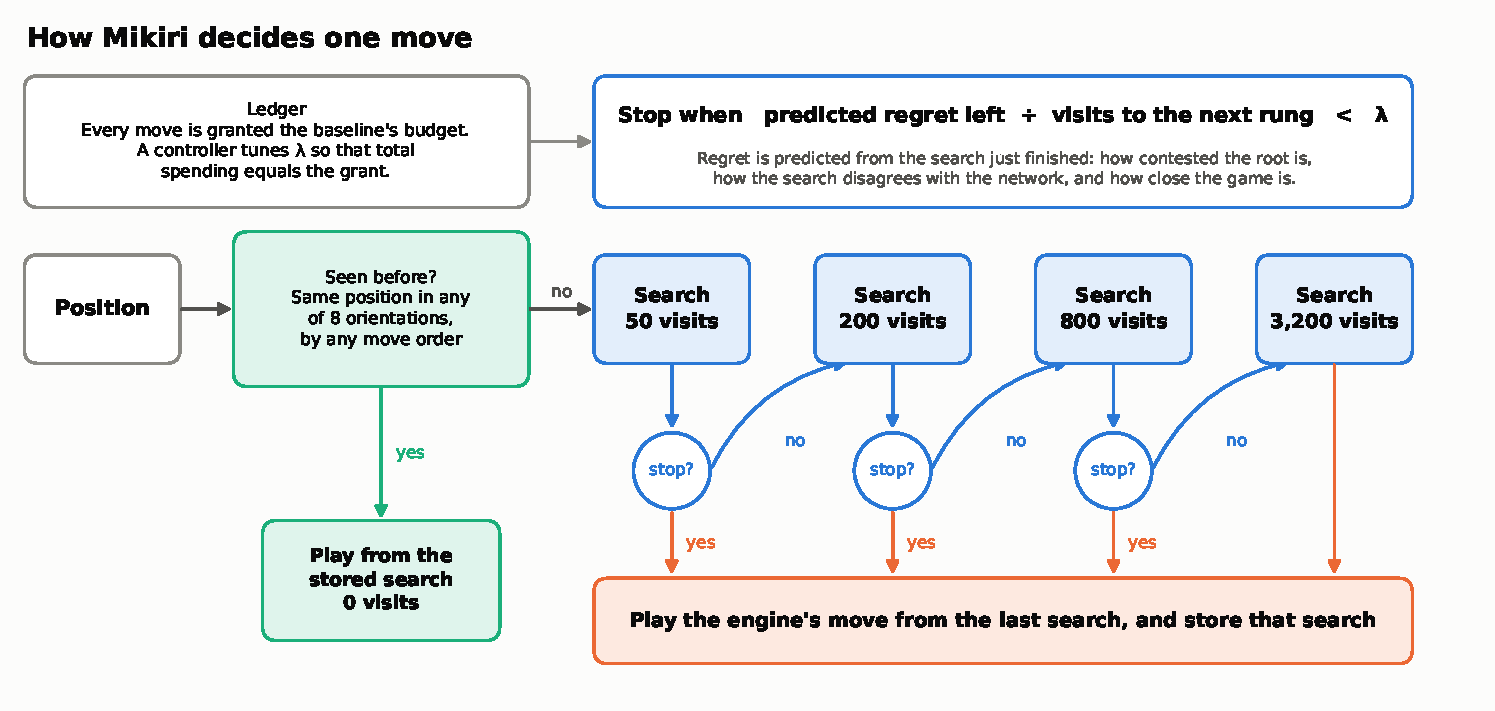
\includegraphics[width=\linewidth]{pipeline}
\caption{How Mikiri decides one move.}
\label{fig:pipeline}
\end{figure}

\subsection{A visit ladder with a learned stop}

Mikiri searches a position at the first rung of a short ladder, for example 50 visits, and asks a model whether the decision is settled. If it is, Mikiri plays. If not, it searches at the next rung (200, then 800, then 3{,}200) and asks again.

The model is a gradient-boosted regression tree ensemble that predicts the regret remaining at the current rung, $\hat r_j(x)$. Its inputs come from the search that just finished, at no extra engine cost:
\begin{itemize}
  \item how contested the root is: visit share of the top two moves, visit entropy, number of moves above 5\% of visits, the margin between the best move's lower confidence bound and the best rival's winrate, and whether the most-visited move is also the highest-valued one;
  \item how the search disagrees with the network: prior of the chosen move, whether it is the top-prior move, the KL divergence from prior to visit distribution, and the gap between the raw network winrate and the searched winrate;
  \item what is at stake: root winrate, its distance from 50\%, score lead, and the spread of score among the leading moves;
  \item KataGo's own raw-network predictions of its short-term winrate and score error;
  \item game phase and the logarithm of visits;
  \item from the second rung on, what changed since the previous rung: whether the best move changed, how many times it has changed so far, and the change in winrate, top-move share, and confidence margin.
\end{itemize}

Mikiri stops at rung $j$ when
\begin{equation}
  \frac{\hat r_j(x)}{v_{j+1}-v_j} \;<\; \lambda .
\end{equation}
The rule comes from a constrained problem. Let a stopping policy $\pi$ stop position $s$ at rung $\pi(s)$. We want
\begin{equation}
  \min_\pi \; \mathbb{E}\bigl[r_{\pi(s)}(s)\bigr] \quad \text{subject to} \quad \mathbb{E}\bigl[v_{\pi(s)}\bigr] \le B .
\end{equation}
With a multiplier $\lambda$ on the constraint the problem separates over positions, each minimising $r_k(s)+\lambda v_k$. At rung $j$ the visits already spent cannot be recovered, and continuing by one rung is worthwhile exactly when $\mathbb{E}[r_j-r_{j+1}\mid x] > \lambda\,(v_{j+1}-v_j)$. The reduction $r_j-r_{j+1}$ is at most $r_j$, and replacing it with a prediction of the regret remaining gives the rule above. Section~\ref{sec:targets} tests the alternatives this derivation suggests, including predicting the reduction itself, and finds that remaining regret is the best target in practice.

The left side is the regret still on the table per visit needed to reach the next rung. A single $\lambda$ then trades winrate against visits at the same rate everywhere on the ladder: going from 800 to 3{,}200 visits requires four times the stake that going from 200 to 800 does. Without this scaling a long ladder spends most of its budget on a handful of positions that no amount of search resolves (Section~\ref{sec:offline}).

The model is trained on the ladder dataset with all non-final rungs pooled. Every offline number we report is cross-fitted: games are split into five folds, and each position is scored by a model that never saw any position from its game. The deployed model is trained on all games and stored as JSON trees evaluated in NumPy.

\subsection{Exact search memory}

Every search Mikiri finishes within the first 80 moves of a game is stored under the position's symmetry-canonical key. When a later game reaches the same position, in any of its eight orientations and by any move order, Mikiri plays from the stored search and spends nothing. The stored result is a search of exactly this position, at the budget Mikiri's own stopping rule chose for it, so a hit gives up nothing in quality.

Entries that keep being hit are worth more than their first search. After each game, if the ledger (below) shows a surplus, Mikiri re-searches the most frequently hit entries at a larger budget and replaces them.

\subsection{A ledger}

To compare fairly with an engine that spends $b$ visits on every move, Mikiri is granted $b$ visits for each move it makes and may never spend more than it has been granted. Memory hits and early stops leave part of the grant unspent. A controller adjusts $\lambda$ after every game so that cumulative spending tracks the cumulative grant, which turns visits saved on known or easy positions into deeper searches on hard ones. Post-game deepening draws on the same ledger. Over a series, Mikiri's total compute, online and offline, is at most the baseline's.

\section{What the ladder dataset shows}
\label{sec:offline}

\subsection{Regret is rare and concentrated}

Table~\ref{tab:uniform} gives the price of a uniform budget. At 200 visits the engine gives up 0.99\% of winrate per move on average, and doubling the budget removes roughly a third of what remains. The average hides the shape. At 200 visits 71\% of positions carry no regret at all: the 200-visit move is the best move we scored. The worst tenth of positions hold 84\% of the total. Regret also depends on when in the game the position occurs. At 200 visits it averages 0.19\% per move over the first 40 moves, 0.74\% from move 40 to 100, and 1.4 to 1.6\% after move 100. The opening is nearly free of search error at these budgets, which will matter for how we interpret memory.

A rule that knew each position's regret and stopped at the first rung with none would match uniform search at twelve times the visits at a 200-visit budget (last column of Table~\ref{tab:frontier}). That is the room available to any stopping rule on this ladder.

\begin{table}[t]
\centering\small
\begin{tabular}{rrrrr}
\toprule
Visits & Mean regret & Positions with & Regret held by & Move differs from \\
 & (\% winrate) & no regret (\%) & worst 10\% (\%) & 3{,}200-visit move (\%) \\
\midrule
50 & 1.47 & 66 & 78 & 33 \\
100 & 1.19 & 68 & 81 & 30 \\
200 & 0.99 & 71 & 84 & 27 \\
400 & 0.70 & 74 & 86 & 22 \\
800 & 0.48 & 78 & 90 & 17 \\
1{,}600 & 0.30 & 82 & 94 & 11 \\
3{,}200 & 0.17 & 86 & 98 & 0 \\
\bottomrule
\end{tabular}

\caption{Uniform search on the ladder dataset (6{,}000 positions). Regret is measured against the best move scored by an independent forced search.}
\label{tab:uniform}
\end{table}

\subsection{No single signal finds it}

Table~\ref{tab:auc} asks how well individual search statistics rank positions by whether more than 0.5\% of winrate remains on the table. The measures of how contested the root is (top move's visit share, the margin between the best move's lower confidence bound and its best rival) reach an AUC of about 0.74. KataGo's own prediction of its short-term winrate error, a signal it uses inside the tree to weight playouts, reaches 0.58 to 0.60 as a predictor of whether the root decision will improve. The classical time-management cue, that the most-visited move is not the highest-valued one \citep{huang2010time}, is weaker still at 0.59 to 0.61. Contested positions are common, and most of them are contested between moves of nearly equal value, where being wrong costs nothing.

\begin{table}[t]
\centering\small
\begin{tabular}{lrrr}
\toprule
Signal & 50 & 200 & 800 \\
\midrule
Top move's visit share & 0.75 & 0.74 & 0.74 \\
LCB margin & 0.74 & 0.73 & 0.73 \\
v1 entropy gate & 0.73 & 0.73 & 0.74 \\
KL(visits, prior) & 0.65 & 0.63 & 0.61 \\
Most-visited is not best-valued & 0.60 & 0.59 & 0.61 \\
KataGo's predicted winrate error & 0.58 & 0.58 & 0.60 \\
Searched minus raw winrate & 0.57 & 0.56 & 0.56 \\
\bottomrule
\end{tabular}

\caption{AUC for ranking positions by remaining regret above 0.5\%, from the search at 50, 200, and 800 visits.}
\label{tab:auc}
\end{table}

\subsection{A learned stop on a ladder beats uniform search by 1.7 to 1.9 times}

Table~\ref{tab:frontier} is the main offline result. With the 50, 200, 800, 3{,}200 ladder and a mean cost of 200 visits, the learned stopper gives up 0.75\% of winrate per move. Uniform search needs 358 visits to do as well, a multiplier of 1.80. The multiplier stays between 1.69 and 1.88 for mean budgets from 100 to 800 visits. If every restarted search is charged in full, so that reaching the 800-visit rung costs $50+200+800$, the multiplier is 1.29 to 1.51.

\begin{table}[t]
\centering\small
\begin{tabular}{rrrrrrr}
\toprule
Mean & Uniform & Stopper & Equivalent & \multicolumn{2}{c}{Multiplier} & Oracle \\
visits & regret (\%) & regret (\%) & uniform visits & continuation & restart & multiplier \\
\midrule
100 & 1.19 & 1.03 & 173 & 1.76 & 1.51 & 5.5 \\
150 & 1.07 & 0.87 & 265 & 1.79 & 1.47 & 9.6 \\
200 & 0.99 & 0.75 & 358 & 1.80 & 1.44 & 12.1 \\
300 & 0.82 & 0.60 & 544 & 1.88 & 1.47 & 10.9 \\
400 & 0.70 & 0.53 & 692 & 1.75 & 1.36 & 8.1 \\
600 & 0.57 & 0.41 & 1072 & 1.80 & 1.38 & 5.7 \\
800 & 0.48 & 0.35 & 1332 & 1.69 & 1.29 & 5.7 \\
\bottomrule
\end{tabular}

\caption{Learned stopping on the 50/200/800/3{,}200 ladder, cross-fitted by game. \emph{Equivalent uniform visits} is the fixed budget with the same mean regret. The oracle stops with knowledge of the true regret.}
\label{tab:frontier}
\end{table}

\subsection{The ladder and the rate rule do most of the work}

Table~\ref{tab:rules} runs hand-written stopping signals through the same ladder. Two things stand out. First, a flat threshold is harmful for most signals: v1's entropy gate with a flat threshold reaches a multiplier of 0.63 at 200 visits, which is worse than not gating at all, and random stopping is far worse. \citet{lan2021learning} made the same observation about random stopping. Second, dividing the score by the visits needed to reach the next rung turns the same signals into gains. The LCB margin alone, with no learning, reaches 1.45 at 200 visits.

\begin{table}[t]
\centering\small
\begin{tabular}{lrrrr}
\toprule
 & \multicolumn{2}{c}{Flat threshold} & \multicolumn{2}{c}{Rate rule} \\
Stopping signal & 200 visits & 400 visits & 200 visits & 400 visits \\
\midrule
Random stopping & 0.44 & 0.29 & 0.71 & 0.69 \\
Most-visited is not best-valued & 0.55 & 0.60 & 0.58 & 0.77 \\
v1 entropy gate & 0.63 & 0.76 & 1.16 & 1.28 \\
LCB margin & 1.13 & 0.86 & 1.45 & 1.00 \\
\midrule
Learned stopper & 1.41 & 1.22 & 1.82 & 1.77 \\
\bottomrule
\end{tabular}

\caption{Compute multipliers (continuation cost) for stopping signals on the 50/200/800/3{,}200 ladder. Values below 1 are worse than uniform search.}
\label{tab:rules}
\end{table}

\section{Matches}
\label{sec:matches}

All matches in this section are played against KataGo at a fixed budget, from the empty board, with alternating colours and KataGo's default move sampling for both players unless noted. Table~\ref{tab:matches} lists every match we ran.

\begin{table}[t]
\centering\footnotesize
\setlength{\tabcolsep}{4pt}
\begin{tabular}{llrrrrrr}
\toprule
Player & Opponent & Games & W--L--D & Elo (95\% interval) & Visits & Restart & Evals \\
\midrule
KataGo 100 visits & KataGo 200 & 400 & 77--301--22 & $-220$ ($-262$ to $-181$) & 100 & 100 & 40/71 \\
KataGo 200 visits & KataGo 200 & 400 & 185--183--32 & $+2$ ($-30$ to $+35$) & 200 & 200 & 76/76 \\
KataGo 283 visits & KataGo 200 & 400 & 247--126--27 & $+108$ ($+76$ to $+143$) & 283 & 283 & 98/73 \\
KataGo 400 visits & KataGo 200 & 400 & 310--73--17 & $+237$ ($+198$ to $+280$) & 400 & 400 & 132/73 \\
DataGo: stopper & KataGo 200 & 1000 & 586--325--89 & $+93$ ($+72$ to $+114$) & 160 & 197 & 80/74 \\
DataGo: stopper, paired openings, no sampling & KataGo 200 & 800 & 561--183--56 & $+178$ ($+153$ to $+205$) & 200 & 250 & 115/96 \\
\bottomrule
\end{tabular}

\caption{All matches. \emph{Visits} is the mean size of the deepest search per move, \emph{Restart} counts every search requested, and \emph{Evals} is network evaluations per move for the player and for its opponent, read from each engine's log.}
\label{tab:matches}
\end{table}

\subsection{What a visit is worth}

To read the other results we first need the exchange rate between compute and strength in this setting. KataGo against itself at 200 visits scores \unisameScore\% over \unisameGames{} games ($\unisameElo$ Elo, $\unisameEloLo$ to $\unisameEloHi$), which checks that the harness has no side bias. At 100 visits it loses $\unihalfElo$ Elo to the 200-visit engine, at 283 visits it gains $\unirootElo$, and at 400 visits $\unidoubleElo$. A doubling is worth about 230 Elo here. In network evaluations the uniform engine runs \unihalfEvals, \unisameEvals, \unirootEvals, and \unidoubleEvals{} per move at the four budgets: fewer than its visits, because consecutive searches share cached evaluations.

\subsection{The stopping rule at equal visits and at equal evaluations}

With the ladder 50, 200, 800, 3{,}200 and the controller holding its mean at the opponent's budget, DataGo scores \mainScore\% over \mainGames{} games (\mainRecord), a gain of $\mainElo$ Elo (95\% interval $\mainEloLo$ to $\mainEloHi$), at \mainVisits{} visits per move. Counting every restarted search it requested \mainRestart{} visits per move, and it ran \mainEvals{} network evaluations per move to KataGo's \mainBaseEvals.

Visits understate DataGo's cost in one respect. A fixed-budget engine re-meets much of its previous tree on the next move and finds those evaluations cached. DataGo's searches vary in size, so less carries over. The strictest comparison therefore matches network evaluations. We reran the match with DataGo granted 160 visits per move. It then ran \strictEvals{} evaluations per move to KataGo's \strictBaseEvals{} and scored \strictScore\% over \strictGames{} games (\strictRecord), a gain of $\strictElo$ Elo ($\strictEloLo$ to $\strictEloHi$).

Figure~\ref{fig:elo} places these results against the uniform curve under all three measures of compute.

\begin{figure}[t]
\centering
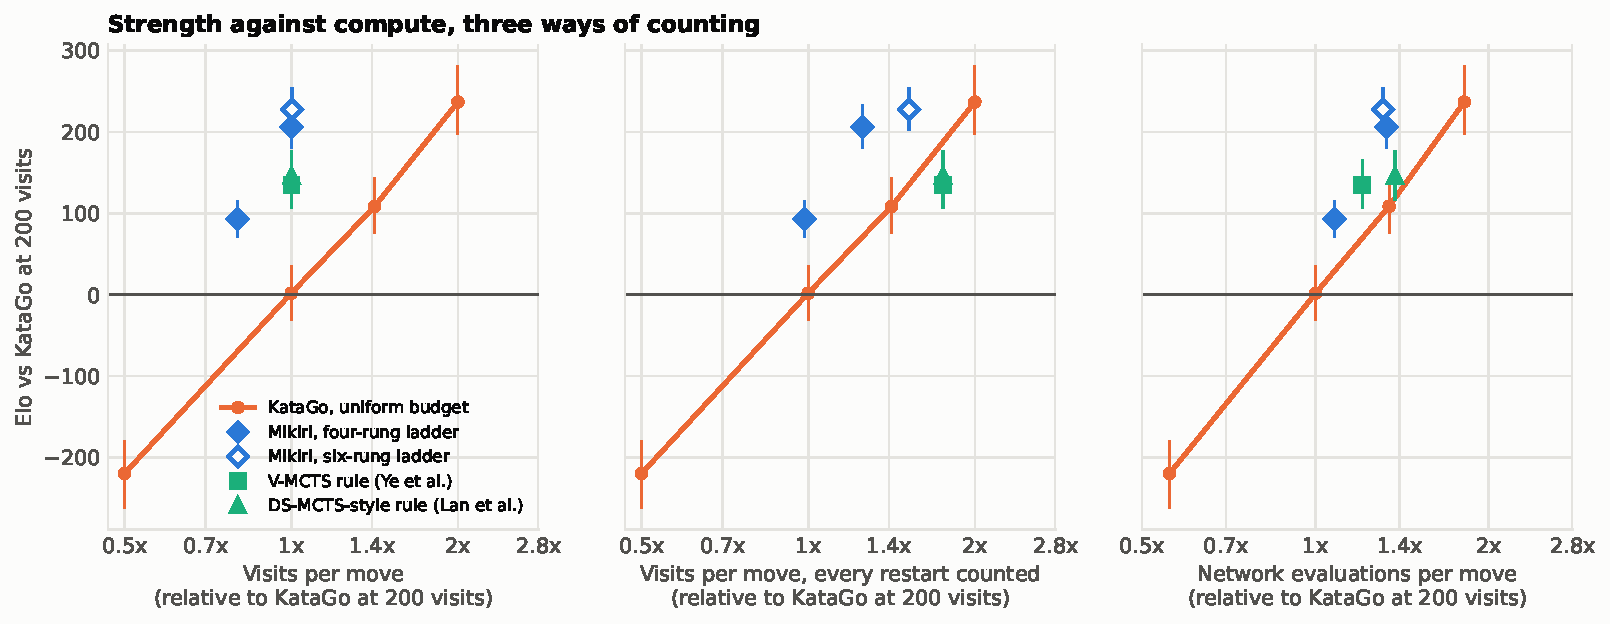
\includegraphics[width=\linewidth]{elo_vs_compute}
\caption{Elo against KataGo at 200 visits, as a function of compute relative to that baseline, counted three ways. The line is KataGo at uniform budgets. Bars are 95\% intervals.}
\label{fig:elo}
\end{figure}

\subsection{Without move sampling}

KataGo's default play samples among well-visited moves early in the game. A search that stops when one move dominates has sharper visit counts than a fixed-budget search, so sampling could favour DataGo for reasons unrelated to search quality. To rule this out we sampled 400 balanced openings of 12 moves, played each twice with colours swapped, and had both players always play their engine's top move. DataGo scores \pairedScore\% over \pairedGames{} games (\pairedRecord), $\pairedElo$ Elo ($\pairedEloLo$ to $\pairedEloHi$), at \pairedVisits{} visits per move.

\subsection{Where the visits go}

Figure~\ref{fig:profile} shows DataGo's spending in the main match. It uses well under the budget in the opening, where Section~\ref{sec:offline} found almost no regret to recover, and more than the budget through the middle game. It also spends by stakes: least when it believes the game is decided and most when the game is in the balance. Neither behaviour was programmed. Both follow from predicting regret in winrate units.

\begin{figure}[t]
\centering
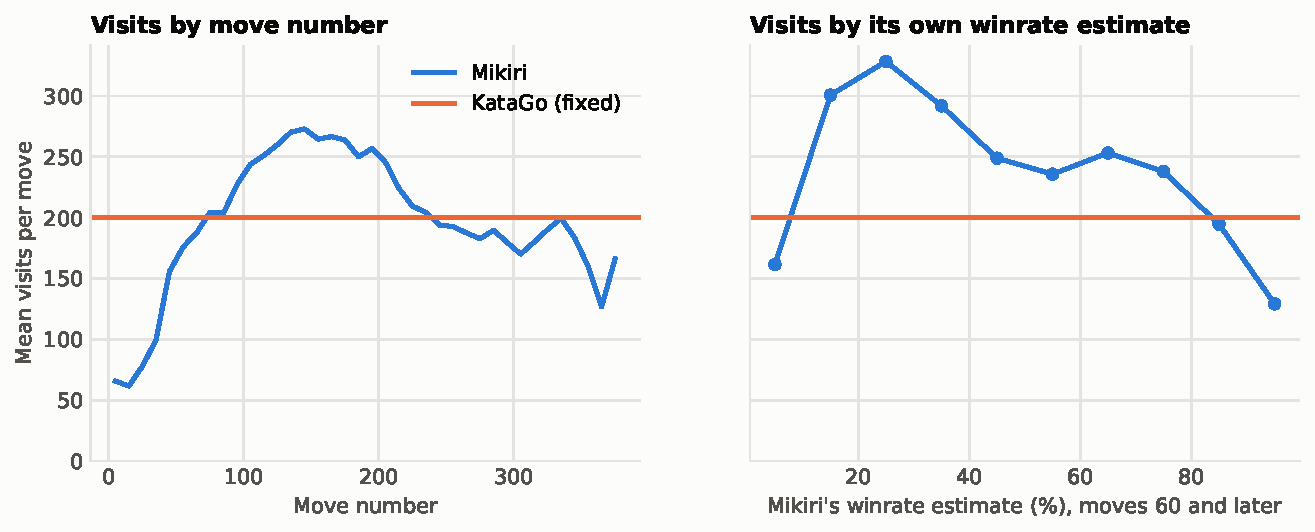
\includegraphics[width=\linewidth]{profile_main}
\caption{Mean visits per DataGo move in the main match, by move number and by DataGo's own winrate estimate.}
\label{fig:profile}
\end{figure}

\subsection{Memory}

With memory alone and no stopper, DataGo is KataGo with an opening book that fills itself. Over \memonlyGames{} games it served \memonlyHitRate\% of its moves from memory (\memonlyHitLate\% in the second half of the series), averaged \memonlyVisits{} visits per move, and scored \memonlyScore\% ($\memonlyElo$ Elo, $\memonlyEloLo$ to $\memonlyEloHi$).

The full system combines memory with the stopper and lets the controller reinvest what memory saves. Over \fullGames{} games it scores \fullScore\% (\fullRecord), $\fullElo$ Elo ($\fullEloLo$ to $\fullEloHi$), at \fullVisits{} visits and \fullEvals{} evaluations per move against \fullBaseEvals, with \fullHitRate\% of moves served from a memory that grew to \fullMemory{} positions.

\subsection{Other budgets, a longer ladder, another network, other boards}

The same model, trained once on 19$\times$19 positions from the b18 network, was run without retraining in six further settings.
\begin{itemize}
\item \textbf{Budgets.} Against KataGo at 100, 400, and 800 visits, at matched visits, DataGo gains $\bhundredElo$ ($\bhundredEloLo$ to $\bhundredEloHi$), $\bfourElo$ ($\bfourEloLo$ to $\bfourEloHi$), and $\beightElo$ ($\beightEloLo$ to $\beightEloHi$) Elo.
\item \textbf{Longer ladder.} The six-rung ladder 50, 200, 400, 800, 1{,}600, 3{,}200, the best offline by continuation cost, gains $\longElo$ ($\longEloLo$ to $\longEloHi$) Elo at \longVisits{} visits, \longRestart{} restart visits, and \longEvals{} evaluations per move.
\item \textbf{A stronger network.} On the 28-block network, with both players using it, DataGo gains $\bignetElo$ ($\bignetEloLo$ to $\bignetEloHi$) Elo.
\item \textbf{Smaller boards.} On 13$\times$13 and 9$\times$9 it gains $\thirteenElo$ ($\thirteenEloLo$ to $\thirteenEloHi$) and $\nineElo$ ($\nineEloLo$ to $\nineEloHi$) Elo.
\end{itemize}

\section{What a frozen engine can and cannot retrieve}
\label{sec:retrieval}

\subsection{Exact positions recur often}
\label{sec:reuse}

How much could an exact-match memory ever serve? We replayed the 300 self-play games behind the ladder dataset in order and asked, for each position, whether its symmetry-canonical key had already occurred in an earlier game. Figure~\ref{fig:reuse} shows the answer for the second half of the games, when the memory holds 150 to 300 games. A position at move 10 had been seen before 86\% of the time, at move 20 51\% of the time, and at move 30 30\% of the time. Games stayed on known ground for 24 moves on average, and one for 108. Over whole games, 11.5\% of all positions were repeats.

These games used a higher early move temperature (0.8) than KataGo's default (0.5), so they are more varied than default play. The reuse rate is large for two reasons: a strong engine's opening choices are concentrated on a few lines, and canonicalising over the eight symmetries and over move order merges what look like different games.

\begin{figure}[t]
\centering
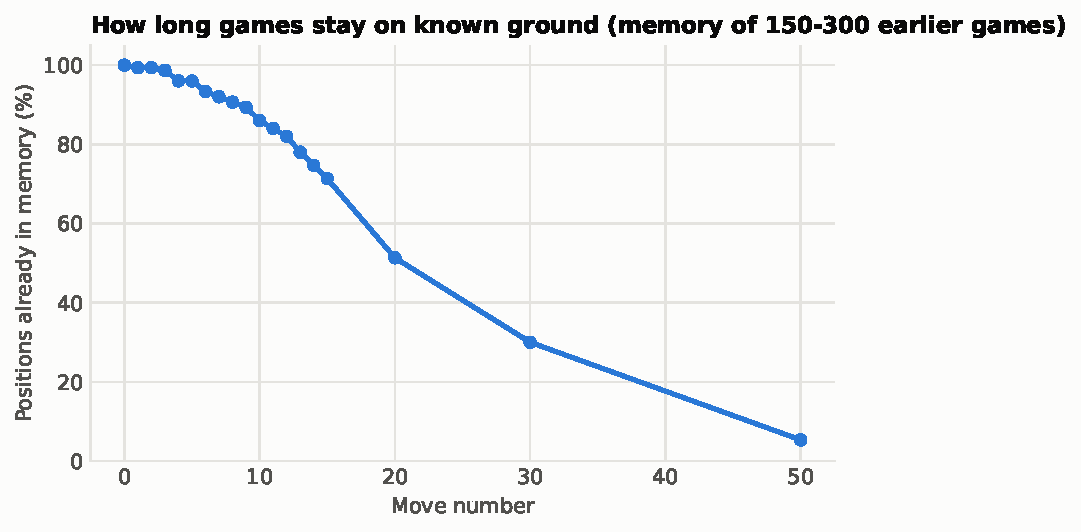
\includegraphics[width=0.62\linewidth]{reuse}
\caption{Share of positions whose canonical key had already occurred in an earlier game, by move number, with a memory of 150 to 300 earlier games.}
\label{fig:reuse}
\end{figure}

\subsection{Near matches do not transfer}
\label{sec:approx}

The first version of DataGo was designed around approximate retrieval: find stored positions that resemble the current one and reuse their analysis. We tested the idea directly. Each position in the ladder dataset is embedded with KataGo's raw policy and ownership maps, compared against every position from other games in all eight orientations, and matched to its nearest neighbours by cosine similarity. A neighbour's 3{,}200-visit move is mapped through the aligning symmetry and offered as a proposal.

Proposals matter in the 1{,}605 positions (27\%) where the 200-visit move differs from the 3{,}200-visit move. There the nearest neighbour's move is the 3{,}200-visit move 5.5\% of the time, and one of five neighbours has it 7.8\% of the time. The policy network's highest-prior alternative to the 200-visit move is right 43\% of the time, and one of its top five 85\%. An index of stored searches is a much worse source of candidate moves than the network the engine already carries.

Figure~\ref{fig:similarity} shows why. A neighbour's best move is this position's best move in 96\% of cases when the similarity exceeds 0.999, which in practice means the same position. Agreement is 86\% between 0.97 and 0.999, 27\% between 0.90 and 0.97, 11\% between 0.8 and 0.9, and under 4\% below that. After move 20 the median nearest-neighbour similarity is 0.75 or lower. Retrieval is useful exactly where the exact key already finds the position, and nowhere else.

The same holds for deciding when to think. The similarity-weighted regret of a position's five nearest neighbours predicts its own regret with an AUC of 0.55. The search's own confidence margin reaches 0.73.

We do not claim that approximate retrieval cannot help Go engines. \citet{humphreys2022retrieval} show that it can when the network is trained to read its neighbours and the index holds tens of millions of positions. Our index holds 6{,}000, and our network is frozen. Within those limits the result is unambiguous, and it matches what is known about Go: \citet{lan2022alphazero} change a strong engine's move by adding two stones that should not matter.

\begin{figure}[t]
\centering
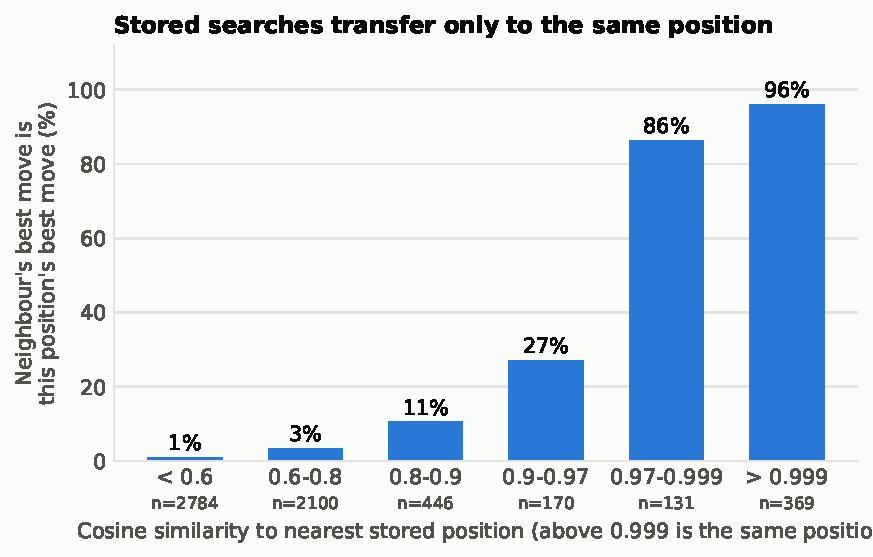
\includegraphics[width=0.62\linewidth]{similarity}
\caption{How often the nearest stored position's 3{,}200-visit move is also this position's, by embedding similarity. Numbers under the bars are position counts.}
\label{fig:similarity}
\end{figure}

\section{Limits}
\label{sec:limits}

\paragraph{One engine family, low budgets.}
All results use KataGo networks at mean budgets of 100 to 800 visits per move. Elo per doubling of visits is steep in this range (about 230 at 200 visits in our matches), which is what makes reallocation valuable. At tournament budgets of tens of thousands of visits the curve is flatter, errors are rarer, and we have not measured what remains to be gained.

\paragraph{The yardstick is a search.}
Regret is defined by 1{,}600-visit forced searches, which are themselves imperfect. They are applied identically to every move and to every policy, so comparisons between policies are fair, but the absolute regret numbers inherit the engine's blind spots. The match results do not depend on the yardstick.

\paragraph{Most of the headroom is out of reach of search statistics.}
The oracle multiplier at 200 visits is 12; the learned stopper reaches 1.8. Among positions with more than 0.5\% regret at 200 visits, 57\% of the regret sits on a best move that had received under 10\% of the visits, and 12\% on one that had received under 1\%. A stopping rule that reads the search cannot see a move the search has not looked at. Closing this gap needs a different source of candidates. Section~\ref{sec:approx} shows that a similarity index is not one.

\paragraph{Memory is an opening book.}
Exact reuse is confined to the first few dozen moves, where search error at these budgets is already small. It saves visits, and in a long-running engine process it saves almost no network evaluations, since the engine's own cache covers the same positions. Against opponents with a wider opening repertoire than KataGo's, hit rates will be lower than ours.

\paragraph{The opponent is cooperative.}
Adversarial policies defeat KataGo at any budget we could afford \citep{wang2023adversarial,tseng2025can}. DataGo reads the same network and the same search, and would stop early with full confidence in exactly the positions those attacks construct.

\paragraph{No direct comparison with AlphaGo.}
AlphaGo and AlphaGo Zero \citep{silver2016mastering,silver2017mastering} are not available to play. KataGo's public networks are among the strongest Go engines anyone can run, so they are the baseline here. What we show is an improvement over that baseline at equal compute.

\section{Conclusion}

A frozen Go engine leaves most of a doubling of search on the table by spending visits uniformly. A small learned rule recovers it, and the part of the rule that matters most is the price it puts on continuing: divide the stake by the cost of the next rung, and signals that were worse than no gate become gains. The same engine cannot be helped by analyses of similar positions, and an exact memory of its own past searches saves visits that its evaluation cache had already made cheap.

We think the more general lesson is about measurement. A search cannot grade itself. Once a yardstick independent of the search exists, questions that looked settled, such as whether a modern engine has anything left to gain from time management, turn out to have numbers attached, and the numbers can be checked against games before the games are played. The testbed, the dataset, every model and every game record are released so that others can check ours.


\section*{Acknowledgments}
The first version of this project, DataGo, was a team project with Benjamin Huh, Jason Peng, Olir Eswaramoorthy, David Roos, and Victor Lun Pun, whose questions about uncertainty gating and reuse of deep searches this work takes up. Its code and report are preserved in the repository under \texttt{legacy/}. Experiments ran on the Dartmouth LISP Lab's machines. KataGo and its networks are the work of David J. Wu and the KataGo community.

\bibliographystyle{plainnat}
\bibliography{refs}

\appendix

\section{Training the stopper}
\label{app:training}

The stopper is a gradient-boosted regression tree ensemble (150 trees of depth 3, learning rate 0.05, row subsampling 0.8, at least 30 samples per leaf) fitted to the square root of regret, with all non-final rungs of the ladder pooled. Its prediction is squared before use. Figure~\ref{fig:training} shows the fit and its dependence on data. Held-out error stops improving at about 100 trees.

\begin{figure}[h]
\centering
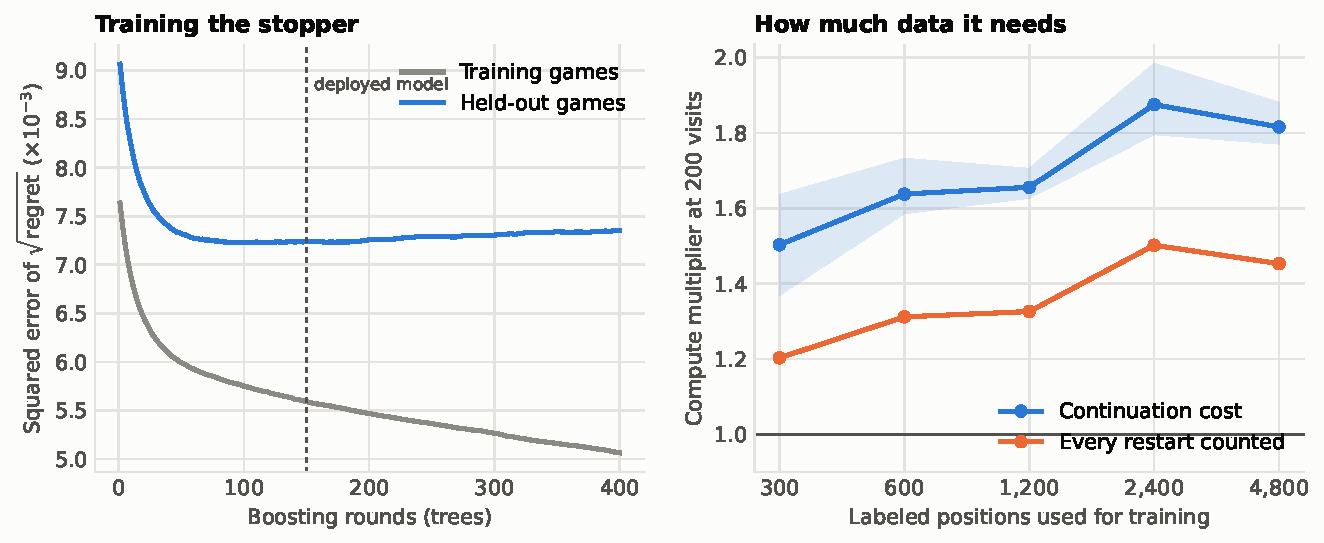
\includegraphics[width=\linewidth]{training}
\caption{Left: squared error on training and held-out games as trees are added. Right: compute multiplier at a 200-visit budget against the number of labeled positions used for training. The band is the range over three draws of training games.}
\label{fig:training}
\end{figure}

Figure~\ref{fig:diagnostics} shows that the score orders held-out positions correctly: realized regret rises from 0.02\% of winrate in the lowest decile of predicted stake to 4.2\% in the highest. The squared prediction underestimates the level of regret, since it estimates a typical value on the square-root scale. This does not affect play, because only the ordering and a controller-tuned threshold are used. The model relies mostly on one feature, the product of how undecided the game is and how far the best rival's winrate exceeds the chosen move's lower confidence bound.

\begin{figure}[h]
\centering
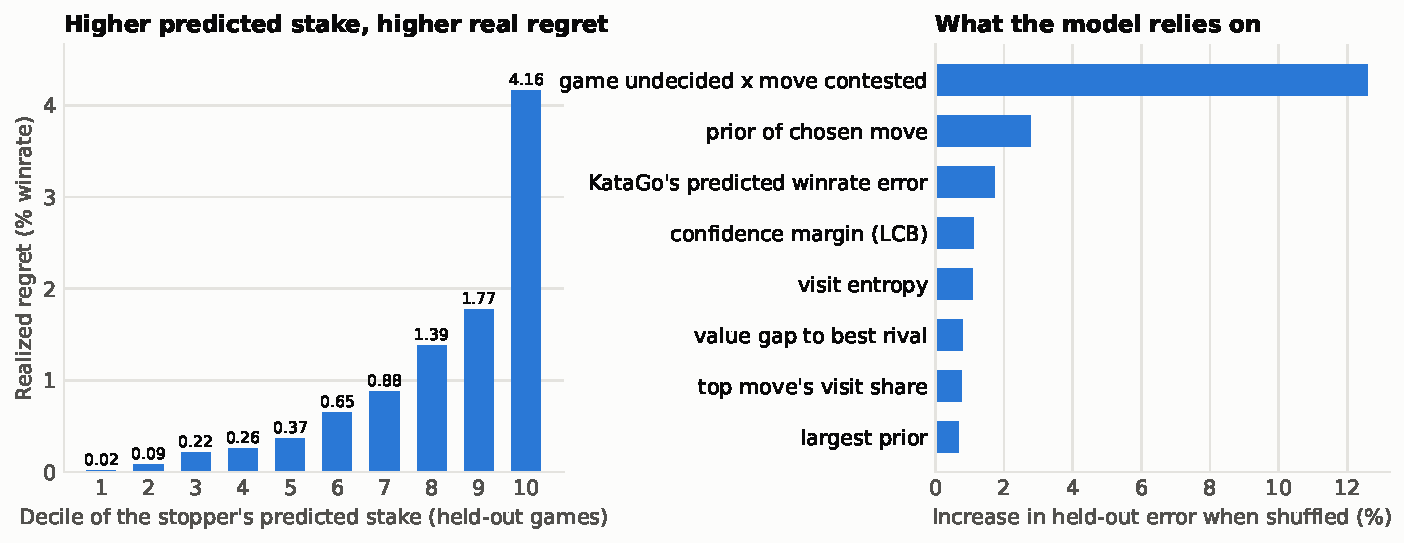
\includegraphics[width=\linewidth]{stopper_diagnostics}
\caption{Left: realized regret by decile of the stopper's score, on held-out games. Right: increase in held-out error when one feature is shuffled.}
\label{fig:diagnostics}
\end{figure}

Table~\ref{tab:ablation} lists the ablations. Each entry is the compute multiplier by continuation cost, with the multiplier under restart accounting in parentheses, averaged over three assignments of games to folds.

\begin{table}[h]
\centering\footnotesize
\begin{tabular}{lrrrr}
\toprule
Variant & 100 & 200 & 400 & 800 \\
\midrule
Full model & 1.81 (1.56) & 1.82 (1.46) & 1.77 (1.37) & 1.64 (1.25) \\
Regret target (no square root) & 1.69 (1.45) & 1.74 (1.39) & 1.64 (1.27) & 1.49 (1.13) \\
Flat threshold (no rate rule) & 1.34 (1.16) & 1.41 (1.13) & 1.22 (0.94) & 1.31 (1.00) \\
No trajectory features & 1.80 (1.55) & 1.82 (1.46) & 1.75 (1.35) & 1.63 (1.24) \\
No KataGo raw error features & 1.76 (1.51) & 1.87 (1.50) & 1.70 (1.31) & 1.62 (1.23) \\
Seven core features & 1.70 (1.46) & 1.73 (1.39) & 1.65 (1.27) & 1.62 (1.23) \\
LCB margin only & 1.44 (1.24) & 1.48 (1.18) & 1.36 (1.05) & 1.07 (0.81) \\
80 trees of depth 2 & 1.76 (1.51) & 1.79 (1.43) & 1.67 (1.29) & 1.60 (1.22) \\
400 trees of depth 3 & 1.74 (1.50) & 1.83 (1.46) & 1.61 (1.25) & 1.58 (1.21) \\
Ladder 50, 200, 800 & 1.86 (1.60) & 1.84 (1.47) & 1.68 (1.30) & 1.00 (0.76) \\
Ladder 100, 400, 1600 & -- & 1.58 (1.36) & 1.55 (1.24) & 1.50 (1.16) \\
Ladder 50, 200, 400, 800, 1600, 3200 & 2.05 (1.62) & 1.98 (1.30) & 1.97 (1.15) & 1.85 (1.01) \\
Ladder 50, 100, 200, 400, 800, 1600, 3200 & 2.04 (1.37) & 2.14 (1.22) & 1.94 (1.04) & 1.86 (0.96) \\
\bottomrule
\end{tabular}

\caption{Stopper ablations at mean budgets of 100, 200, 400, and 800 visits.}
\label{tab:ablation}
\end{table}

\section{Reproducing the results}

The repository contains the ladder dataset, the trained models, every game record, and the scripts that produce each table and figure from them. The dataset took 1.5 GPU-hours to label on one RTX 6000 Ada, and a 1{,}000-game match at 200 visits takes about the same. Training the stopper takes minutes on a laptop CPU. The test suite runs the full pipeline against a small stand-in engine and needs no GPU.

\end{document}
